% Select language used in document (ngerman or english). Automatically
% generated text is translated accordingly.
% use \selectthesislanguage in body.tex to switch to default language

%\documentclass[english, paper]{mmt} % use for BA1
\documentclass[english, bachelorthesis]{mmt} % use for BA2
%\documentclass[ngerman, masterthesis]{mmt} % use for Master thesis


% user added packages
% ----------------------------
\usepackage{subcaption}
% ----------------------------


\usepackage{mathptmx}
\usepackage{graphicx}
\usepackage{times}
\usepackage{subfig}
\usepackage{float}
\usepackage[utf8]{inputenc}
\usepackage{listings}
\usepackage{makecell}
\usepackage[toc,page]{appendix}
\usepackage{hyperref}
\hypersetup{
    colorlinks,
    citecolor=black,
    filecolor=black,
    linkcolor=black,
    urlcolor=black
}
\usepackage{breakurl}

\usepackage{amsmath}
\usepackage[autostyle,german=guillemets]{csquotes}

% moved to cls file. use \selectthesislanguage to switch to default language
%\usepackage[english,ngerman]{babel}

\usepackage{abbrevs}
%% the following solves a bug in the abbrevs package, that adds an empty
%% space after the abbrev
\makeatletter
\renewcommand\maybe@space@{%
  % \@tempswatrue % <= this is in the original
  \maybe@ictrue % <= this is new
  \expandafter   \@tfor
    \expandafter \reserved@a
    \expandafter :%
    \expandafter =%
                 \nospacelist
                 \do \t@st@ic
  % \if@tempswa % <= this is in the original
  \ifmaybe@ic % <= this is new
    \space
  \fi
}
\makeatother
%%


\usepackage{listings}
\usepackage{color}
\definecolor{lightgray}{rgb}{.9,.9,.9}
\definecolor{darkgray}{rgb}{.4,.4,.4}
\definecolor{purple}{rgb}{0.65, 0.12, 0.82}
\lstdefinelanguage{JavaScript}{
  keywords={break, case, catch, continue, debugger, default, delete, do, else, false, finally, for, function, if, in, instanceof, new, null, return, switch, this, throw, true, try, typeof, var, let, const, void, while, with},
  morecomment=[l]{//},
  morecomment=[s]{/*}{*/},
  morestring=[b]',
  morestring=[b]",
  ndkeywords={class, export, boolean, throw, implements, import, this},
  keywordstyle=\color{blue}\bfseries,
  ndkeywordstyle=\color{darkgray}\bfseries,
  identifierstyle=\color{black},
  commentstyle=\color{purple}\ttfamily,
  stringstyle=\color{red}\ttfamily,
  sensitive=true
}

\lstset{
   language=JavaScript,
   backgroundcolor=\color{lightgray},
   extendedchars=true,
   basicstyle=\footnotesize\ttfamily,
   showstringspaces=false,
   showspaces=false,
   numbers=left,
   numberstyle=\footnotesize,
   numbersep=9pt,
   tabsize=2,
   breaklines=true,
   showtabs=false,
   captionpos=b
}

\usepackage[authordate,bibencoding=auto,strict,noibid,backend=biber]{biblatex-chicago}
\bibliography{bibliography}

%% Add configuration options
\newabbrev{\authorname}{Jan Claudio Mikusch}
\newabbrev{\authormail}{jmikusch.mmt-b2017@fh-salzburg.ac.at}
\newabbrev{\titlename}{Non-verbal communication mechanics in cooperative puzzle games}
\newabbrev{\advisor}{MSc Josef Schinwald}
%\newabbrev{\secondadvisor}{Titel Vorname Nachname}
\newabbrev{\thesisdate}{28.06.2020}
\newabbrev{\keywordsenglish}{word1, word2, word3}
\newabbrev{\keywordsgerman}{wort1, wort2, wort3}


%% Paper title.

\title{\titlename}

%% This is how authors are specified in the conference style

%% Author 
\author{ \authorname\\ \scriptsize \authormail \\ \scriptsize 
\ifmmtlanguagegerman FH Salzburg \else Salzburg University of Applied Sciences \fi
}

%% A teaser figure can be included as follows, but is not recommended since
%% the space is now taken up by a full width abstract.
%\teaser{
%  \includegraphics[width=1.5in]{sample.eps}
%  \caption{This can be a teaser image of the thesis.}
%}

%% Abstract section for paper format.
\abstract{
    \ifmmtlanguagegerman 
        \selectlanguage{ngerman}
        Die Zusammenarbeit mehrerer Leute setzt vorraus, das man über irgend eine Art und Weiße miteinander kommunizieren kann. In kooperativen Computerspielen  besteht neben verbalen und physikalischen non-verbalen Kommunikationsmittel zusätzlich virtuelle non-verbale Kommunikationsmittel.
Diese Bachelorarbeit beschreibt sowohl Kommunikationsformen, die in Computerspielen eingesetzt werden, als auch bereits existierende virtuelle Kommunikationsmechaniken, sowie eine Einteilung dieser kooperativen Mechaniken. 
Für die Durchführung einer Studie wurde ein Prototyp gebaut. Dieser Prototyp ist ein netzwerkbasiertes, kooperatives Multiplayer Puzzle-Spiel, welches von zwei Spielern bzw. Spielerinnen in Echtzeit gespielt werden kann. Als im Spiel implementierte Kommunikationsmechaniken dienen vier verschiedene kooperative Mechaniken: verschiedene Arten von Pings, verschiedene Emojis, das Anbringen von permanenten Bodenzeichnungen sowie die Aufzeichnung der Spielerposition, die in einer Schleife nach der Aufnahme abgespielt wird. 
Neben der Spielidee wird auch die Implementierung der Mechaniken beschrieben.
Während einer online-basierten User-Studie haben die Teilnehmer und Teilnehmerinnen 30 Minuten Zeit, alle neun Level zu absolvieren. Dabei ist verbale Kommunikation nicht erlaubt, wodurch die Teilnehmer und Teilnehmerinnen auf die vier implementierten kooperativen Kommunikationsmechaniken angewiesen sind. Ziel dieser Arbeit ist es zu untersuchen, wie die Teilnehmer und Teilnehmerinnen die Mechaniken benutzen, sowie Kommunikationsformen in einen selbstgebauten Prototypen implementiert werden können.
    \else 
        \selectlanguage{english}
        Working together with multiple people has the requirement, that these people are able to communicate with some kind of communication type.
In cooperative computer games, players are able to communicate using verbal and physical non-verbal communication types. However, computer games additionally have the possibility to use virtual types of non-verbal communication, which sometimes cannot be done in the real world.
This bachelor thesis describes communication types that can be used within computer games, as well as already existing game mechanics and their classification.
To conduct a study, a prototype was built. This prototype is a network-based cooperative multiplayer puzzle game, which can be played by two players in real time. For implemented communication mechanics, players are able to use four different types of communication tools: different kinds of pings, various types of emojis, permanent placeable decals, as well as the recording of the player character position, which is then played in a loop after the recording has finished.
During an online-based user study, attendees have 30 minutes to pass all nine levels. 
Verbal communication is not allowed during the testing. For communication, players are only able to use the given communication mechanics.
The aim of this thesis is to investigate, how players are using the provided cooperative communication mechanics, as well as how game communication mechanics can be implemented in a self made computer game. 
    \fi
}

%%%%%%%%%%%%%%%%%%%%%%%%%%%%%%%%%%%%%%%%%%%%%%%%%%%%%%%%%%%%%%%%
%%%%%%%%%%%%%%%%%%%%%% START OF THE PAPER %%%%%%%%%%%%%%%%%%%%%%
%%%%%%%%%%%%%%%%%%%%%%%%%%%%%%%%%%%%%%%%%%%%%%%%%%%%%%%%%%%%%%%%%

\begin{document}
% TODO switch for english, german
\selectthesislanguage

\pagenumbering{gobble}

 % group open
\ifmmtpaper 
\begingroup 
    % is required because paper template messes with sizes
    \fontsize{12}{18}\selectfont        
    \setlength{\parindent}{0pt}
    \setlength{\parskip}{5pt plus 2pt minus 1pt}
    \sectionfont{\fontsize{14}{15}\selectfont}
\fi

    \input{title}        
    \onecolumn           
    
    \pagenumbering{roman}
    
    \newpage
    \input{affidavit}  % comment out for expose

% group closing
\ifmmtpaper
\endgroup
\fi

%\ifmmtpaper\else
    
    \newpage
    \selectlanguage{ngerman}
    \section*{Kurzfassung}
    Die Zusammenarbeit mehrerer Leute setzt vorraus, das man über irgend eine Art und Weiße miteinander kommunizieren kann. In kooperativen Computerspielen  besteht neben verbalen und physikalischen non-verbalen Kommunikationsmittel zusätzlich virtuelle non-verbale Kommunikationsmittel.
Diese Bachelorarbeit beschreibt sowohl Kommunikationsformen, die in Computerspielen eingesetzt werden, als auch bereits existierende virtuelle Kommunikationsmechaniken, sowie eine Einteilung dieser kooperativen Mechaniken. 
Für die Durchführung einer Studie wurde ein Prototyp gebaut. Dieser Prototyp ist ein netzwerkbasiertes, kooperatives Multiplayer Puzzle-Spiel, welches von zwei Spielern bzw. Spielerinnen in Echtzeit gespielt werden kann. Als im Spiel implementierte Kommunikationsmechaniken dienen vier verschiedene kooperative Mechaniken: verschiedene Arten von Pings, verschiedene Emojis, das Anbringen von permanenten Bodenzeichnungen sowie die Aufzeichnung der Spielerposition, die in einer Schleife nach der Aufnahme abgespielt wird. 
Neben der Spielidee wird auch die Implementierung der Mechaniken beschrieben.
Während einer online-basierten User-Studie haben die Teilnehmer und Teilnehmerinnen 30 Minuten Zeit, alle neun Level zu absolvieren. Dabei ist verbale Kommunikation nicht erlaubt, wodurch die Teilnehmer und Teilnehmerinnen auf die vier implementierten kooperativen Kommunikationsmechaniken angewiesen sind. Ziel dieser Arbeit ist es zu untersuchen, wie die Teilnehmer und Teilnehmerinnen die Mechaniken benutzen, sowie Kommunikationsformen in einen selbstgebauten Prototypen implementiert werden können.
    \ifmmtmasterthesis
    
    \vspace*{0.5cm} 
    \textbf{Schlüsselwörter:~} \keywordsgerman
    \fi
    \newpage
    \selectlanguage{english}
    \section*{Abstract}
    Working together with multiple people has the requirement, that these people are able to communicate with some kind of communication type.
In cooperative computer games, players are able to communicate using verbal and physical non-verbal communication types. However, computer games additionally have the possibility to use virtual types of non-verbal communication, which sometimes cannot be done in the real world.
This bachelor thesis describes communication types that can be used within computer games, as well as already existing game mechanics and their classification.
To conduct a study, a prototype was built. This prototype is a network-based cooperative multiplayer puzzle game, which can be played by two players in real time. For implemented communication mechanics, players are able to use four different types of communication tools: different kinds of pings, various types of emojis, permanent placeable decals, as well as the recording of the player character position, which is then played in a loop after the recording has finished.
During an online-based user study, attendees have 30 minutes to pass all nine levels. 
Verbal communication is not allowed during the testing. For communication, players are only able to use the given communication mechanics.
The aim of this thesis is to investigate, how players are using the provided cooperative communication mechanics, as well as how game communication mechanics can be implemented in a self made computer game. 
    \ifmmtmasterthesis
        
    \vspace*{0.5cm} 
    \textbf{Keywords:~} \keywordsenglish
    \fi
    \selectthesislanguage
    
    \newpage
    \tableofcontents
    
    \newpage
    \listoffigures
    \lstlistoflistings
    \listoftables
    
%\fi

\mmtcolumnmode % switch back to column formatting of stylesheet

\maketitle % used for paper formatting

\ifmmtpaper\else
\pagestyle{headings}
\fi
\pagenumbering{arabic}


\section{Introduction}
\label{section:Introduction}
Cooperation is an anchor of our society and a key ability of people who are working, studying and carrying out most leisure activities together to achieve shared goals \autocite{Morschheuser2017HowGame}[169]. A key part of cooperation is communication. To work together, a team has to share information to work towards a common goal.
Cooperative multiplayer computer games have, apart from some exceptions, always a goal, a team is working to achieve, which can be to accomplish a high score, complete a level, win against an enemy team and so on.

The aim of this thesis is to show, how players will interact within a cooperative puzzle game without the possibility to communicate using their voice, in an unfamiliar environment and how non-verbal communication forms can be implemented. 
To provide an unfamiliar game players have never played before, a self-made cooperative puzzle game is created. It implements different non-verbal communication mechanics, enabling players to communicate during play.

Section \ref{section:Communication} shows, how communication is used in computer games, as well what is necessary to share information successfully. Verbal and non-verbal communication forms are described and how common ground influences communication, as well as the meaning of embodiment in games.
Afterwards, the influence and reason of game mechanics for in-game communication is discussed. Additionally, the framework of \textcite{Toups2014ATheory}, which divides cooperative game mechanics into six different types, is described.

In the implementation section \ref{section:Implementation}, the game idea, as well as all game elements are explained. 
The implementation of four cooperative game mechanic types are explained as well. Besides an attention-focusing ping mechanic, an expressive mechanic in form of emojis, environment-modifying decals and the recording of the player position are implemented.
After the theoretical part of the implementation is explained, the following sections describe, how each game element and all communication mechanics are implemented, using Unity as a game engine, together with Photon as a network-multiplayer framework.

The procedure of the study, followed by the study results, shows how players are using the provided communication mechanics. The whole study is done online, without physical contact to and between the participants.


\section{Related Work}
\label{section:Related Work}
There are several studies about performance improvement through cooperative communication.
\textcite{Vaddi2016Investigating2}[45] showed in their study, that communication has a massive impact on the performance of players. Their participants were assigned four different communication conditions. Having the possibility to talk, using in-game mechanics, both and neither of these possibilities.
Results indicated, that the combination of voice and in-game mechanics occurs to be the highest performing condition.

\textcite{Leavitt2016PingGames}[4346] showed in their paper, that virtual team members employ non-verbal communication strategies to improve their performance up to a point for certain crucial actions. But using these mechanics too much, showed a negative impact, resulting in interruption of gameplay actions.
Additionally, \textcite{Wuertz2017Why2}[1978] looked into, why and how people use gesturing tools in a \textit{Multiplayer Online Battle Arena} game (MOBA), and what degree they view them as important for coordinating with teammates to win matches.

\textcite{Cheung2012CommunicationGaming} wrote about the communication channels and awareness cues in co-located collaborative time-critical gaming. They analysed, how players communicate when they need to be highly focused, but have only analysed the collaboration in an co-located setting.
Also \textcite{Williams2007CanCommunity} reports the influence of voice communication into existing online communities.

Regarding the theoretical part of communication, the work of \textcite{Benford2001CollaborativeEnvironments} and \textcite{Maher2011DesignersEnvironments} provided information about collaborative virtual environments.
Also the work of \textcite{Galantucci2012TheHumans} about embodiment within games and the paper about common ground of \textcite{Clark2004GroundingCommunication.} played an important part of theoretical research.


\section{Communication}
\label{section:Communication}
The following subsections discuss what is necessary for communication in multiplayer games.
Human communication can roughly be divided into verbal communication and non-verbal communication \autocite{Kujanpaa2003SupportingAvatars}[2]. 
Apart from that, the reason why common ground is needed for players is discussed. Also the embodiment of players within virtual worlds and the collaborative virtual environment is described.



\subsection{Verbal Communication}
\label{section:Verbal Communication}

People use voice or text for communication, which is known as verbal communication.
Voice however cannot only be used to spread information.
For evolutionary reasons, humans have come to use voice to determine gender, personality, intentions etc. \autocite{Williams2007CanCommunity}[427].

Most massive multiplayer online games use text-based chat systems.
\textcite{Williams2007CanCommunity} say that although text communication lacks vocal and expression-based cues, it allows different kinds of people to connect and interact with each other. As they are unable to see one another and likely less aware of their differences, conversations can be about their mutual interests or activities, being less hampered by restrictive social norms based purely on their demographics \autocite{Williams2007CanCommunity}[428].

With telecommunication and the internet, communication over large distance became possible. Before Voice over IP (VoIP) was invented, players were only able to communicate with each other using text-based communication. Voice chat may, when compared to text, improve the bridging function through the expansion of social cues, bringing communication closer to the presumed gold standard of face to face communication \autocite{Williams2007CanCommunity}[431].

Players use verbal communication in games to maintain mutual understanding, form strategies and share experiences as well as their current game status \autocite{Cheung2012CommunicationGaming}[572].

In fast paced FPS-games, players use callouts for very fast sharing of information. \textcite{Tang2012VerbalGames}[581] found during a study, that these callouts are often eight words or fewer. As a response, players get short answers as feedback.
However, to understand such short phrases, players have to understand the game environment and game mechanics, so they can predict the teammate to understand everything in an appropriate way \autocite{Tang2012VerbalGames}. This is connected to the term common ground in section \ref{section:Common Ground}. Players always have to know the structure of the game, so they can talk about it without too many misunderstandings.

The ability of voice communication is also positively affecting the player performance. \textcite{Vaddi2016Investigating2}[46] showed during a test, that players who can use voice and in-game communication mechanics had the best performance, followed by voice only communication. Potentially as players become more comfortable with the game and its mechanics, the communication mechanics matter even less \autocite{Vaddi2016Investigating2}[46]. Therefore, the verbal communication seems to have an even bigger impact on advanced players.




\subsection{Nonverbal Communication}
\label{section:Nonverbal Communication}

\begin{figure}
    \centering
    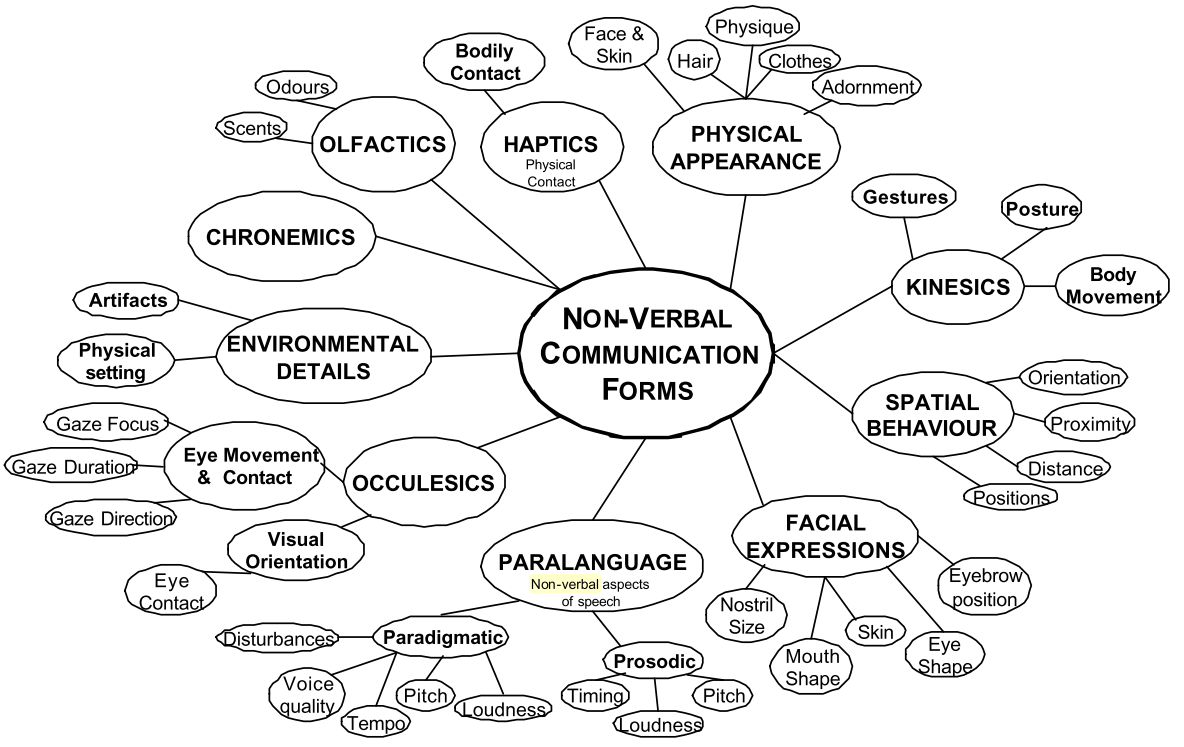
\includegraphics[width=0.95\textwidth]{images/non-verbal_communication_forms.png}
    \caption{ Concept model depicting the non-verbal communication forms
    \break
    \autocite{Manninen2002Non-VerbalSession}[7]. }
    \label{fig:non-verbal communication forms}
\end{figure}

People use non-verbal communication to coordinate actions in all aspects of daily life, including the use of body movements, pointing, touching, gazing, and so on \autocite{Leavitt2016PingGames}[4338].

During fast gameplay in co-located games, \textcite{Cheung2012CommunicationGaming}[576] observed nearly no non-verbal communication, concerning face to face communication.
Looking away would introduce too high risk of awareness or communication breakdowns and removing the hands of the controller could have dire consequences during gameplay \autocite{Cheung2012CommunicationGaming}[576]. Anyway, this physical based non-verbal communication is only feasible during co-located multiplayer games.


In figure \ref{fig:non-verbal communication forms}, many different forms of non-verbal communication forms are displayed. A lot of them can be transferred from physical to virtual space. The visual elements, physical appearance, kinetics and facial expressions can be used to support the design of more communicative computer game avatars \autocite{Kujanpaa2003SupportingAvatars}[6].

Computer games can also have additional non-verbal communication elements, which are not always possible in the physical world. As example, players in Portal 2 can coordinate their actions using ping tools \autocite{Vaddi2015Validating2}[722]. With free hand annotations in Dota 2, players can create a drawing on the minimap \autocite{Wuertz2017Why2}[1979].


\subsubsection{Gestures}

Physical gestures are limited to co-located multiplayer games and players are also often hindered of using them, as removing the hands from the game controller may have negative consequences \autocite{Cheung2012CommunicationGaming}[570]. Besides physical gestures, virtual environments enable players to use virtual gestures as well.

Virtual gestures are gestures within the game, used by an avatar to indicate objects, areas and directions \autocite{Cheung2012CommunicationGaming}[573].
Also pointing with a weapon or shooting at ammunition instead of describing its location is a common scenario \autocite{Cheung2012CommunicationGaming}[573]. Some gestures seem to be already understood by players from their previous gaming experiences, as they do not explain or discuss some virtual gestures \autocite{Cheung2012CommunicationGaming}[574].

\textcite{Wuertz2017Why2} observed during two studies why gestures were created and found six distinct motivations: planning, warning, resource, conflict, help, and emotion.
Therefore, virtual gestures and other virtual non-verbal communication forms can be expanded by implementing mechanics, which enable collaboration. In Section \ref{Cooperative game mechanics}, such cooperative game mechanics are discussed further.

\subsection{Common Ground}
\label{section:Common Ground}

When two people talk with each other, they will assume knowledge about certain things, which means the other one has to be aware of the background information the discussion is about. The example of \textcite{Stalnaker2002CommonGround}[702] is the sentence "The king of France is bald", that presupposes that France has a unique king. This stack of information is called common ground. 

``A representation of the common ground helps to clarify both of the ends of the communicative action by representing the possibilities among which the speaker intends to distinguish, and the means available to the speaker to distinguish between them - the information that must be available in order for the act of uttering certain noises reasonably be taken as an act of trying to get someone to acquire certain information'' \autocite{Stalnaker2002CommonGround}[702].
If a presumption is not known at a certain point, it will come to existence at this certain point, which is called the phenomenon of \textit{presupposition accommodation} \autocite{Stalnaker2002CommonGround}[705].

The start point of the common ground during a conversation can be a common or mutual belief, something everybody knows and everybody knows that the knowledge is also present for everybody else. However, there can be false assumptions, that other people know it as well, which then cannot be counted to common belief.
Since common beliefs and beliefs about common beliefs are derivative from individual beliefs, the way they change in the course of a conversation will be determined by ordinary belief changes \autocite{Stalnaker2002CommonGround}[708].
Therefore, the common belief is not static during a conversion and both types of beliefs will change during the ongoing conversation. This process by which something becomes common ground in virtue of one party recognising that the other takes it to be common ground, is called accommodation \autocite{Stalnaker2002CommonGround}[712]. 
Assumptions one person makes can become part of the common ground of the discussion if it is accepted by others, even if it is only temporary.


\textcite{Clark2004GroundingCommunication.}[222] said that it takes two people to work together for certain things and both have to coordinate the content and process of what they are doing to succeed in it.
In other words, common ground is the basis a conversation needs to be successful. Information is pre-assumed and can differ from others. If that happens, the group has to agree on what they are talking about.  


\subsection{Embodied Communication}
\label{section:Embodied Communication}

Embodying communication entails that the individuals engaged in communication have a body with which they are presented in the world, and that they can only communicate through this body, as opposed to through some kind of direct or indirect way to transfer meaning \autocite{Galantucci2012TheHumans}[229].

This embodiment implies, that partners which can communicate have limited knowledge of what each of them perceives or knows \autocite{Galantucci2012TheHumans}[230]. Therefore, telepathy and automatic shared information is not part of it. Additionally, every player needs to have a different perspective to gather information separately from each other, which can then be shared by communicating. 

According to \textcite{Vaddi2016Investigating2}[42], a player avatar, which is capable of communication through cooperative communication mechanics, offers players a means to communicate in an embodied way.

The player avatar can be seen as a representation of the other player. Thus, teammates will know where the player is currently positioned, where the player is going to, may see what someone is planning, and so on.


\subsection{Collaborative Virtual Environments}
\label{section:Collaborative Virtual Environments}

Collaborative virtual environments (CVE) are virtual worlds shared by participants across a computer network \autocite{Benford2001CollaborativeEnvironments}[79]. In computer games, players are provided a player avatar, which enables players to communicate in a embodied way, described before (Section \ref{section:Embodied Communication}). The game-world itself is a collaborative virtual environment. Players are able to interact with each other, as long as they are part of the same environment.

Players in online multiplayer games are rarely physically side by side. During studies of cooperative work, real-world environment have highlighted the important role of physical space as a resource for negotiating social interaction \autocite{Benford2001CollaborativeEnvironments}[80]. Therefore, CVEs have the potential to take the same part as physical space in virtual communication platforms.
Within this CVEs, avatars present their identity, presence, location and activities, which can be graphically seen by others \autocite{Benford2001CollaborativeEnvironments}[79].
Furthermore \textcite{Maher2011DesignersEnvironments}[3] notes in her work that communication among the participants in a CVE is often about location and viewpoints, allowing individuals to pursue their own tasks as well as have their attention focused on a shared task.


\section{Game mechanics for in-game communication}
\label{section:Game mechanics for in-game communication}
The data analysis of \textcite{Cheung2012CommunicationGaming}[572] revealed that players also rely on implicit awareness of each other’s gameplay status to adjust strategies silently. In their study, participants utilised verbal communication, virtual gestures and physical gestures.
To maintain mutual understanding and to form strategies based on common ground, players talk to each other directly \autocite{Cheung2012CommunicationGaming}[572]. As an example, a player could ask his teammate to split up, so they are able to attack an opponent from two different sides.

Another reason to talk to each other is the exchange for information, where the partner is in possession of information that needs to be shared. For example one player could have seen an enemy, but his teammate has no knowledge of this yet. As the writing of \textcite{Cheung2012CommunicationGaming}[573] says, a player can verbally announce their own status or actions that they thought would affect their partner. This could also effect the status of a player, for example the amount of health only the player itself is able to see.

\textcite{Cheung2012CommunicationGaming}[573] mentions that the announcing of points of interest, for example an spotted treasure, is often followed by or accompanied with a virtual gesture. They will point with their weapon onto objects they want to indicate, shoot at it or somehow use other possible gestures hey can use. They can even use they player characters position and running direction or rotation to indicate a direction.
In most situations virtual gestures provide a faster means to convey information than through verbal communication \autocite{Cheung2012CommunicationGaming}[573]. This virtual gestures are normally already understood by both players through previously gaming experiences, as they do not need to discuss the meaning of the gesture first \autocite{Cheung2012CommunicationGaming}[574].

Next to the communication channels \textcite{Cheung2012CommunicationGaming}[574] described, the awareness cues, which are categorised into central cues and peripheral cues, are also very important to maintain the awareness of the environment of each other in the game. 
\begin{itemize}
    \item Central Cues 
    
    Central cues are information the player is able to gain on his own through his own screen \autocite{Cheung2012CommunicationGaming}[574]. This indicates the current position, the direction and the remaining health of a player and each teammate. This also includes that a teammate is standing before an interact-able item.
    \item Peripheral Cues
    
    Peripheral cues are information, which are not restricted to functionality provided by the game \autocite{Cheung2012CommunicationGaming}[574]. Most of these cues are relating to co-location multiplayer games where a split-screen is used for example. A player could hear the other character screaming, which could indicate that the other player is in danger. Also a look onto the screen of a follow player counts to peripheral cues as stated by \textcite{Cheung2012CommunicationGaming}[574].
\end{itemize}

The third communication channel \textcite{Cheung2012CommunicationGaming}[572] described are physical gestures. Co-located players are able to point onto the screen with their hands, as well as other physical gestures such as waving. As this study not about co-location games, physical gestures are negligible, because it is not possible to use them in a network-based game per design.



\iffalse
----------------------
In online games, physical gestures cannot be used, because the players are not physically next
to each other. Virtual gestures can reach from using in-game avatar movement to using the
characters rotation and their utility (for example weapon) direction to point on certain things
(Cheung, Chang, and Scott 2012)[572]. Communication is not limited to direct methods of
transferring meaning (Toups et al. 2014)[258]. With changing environments, which includes
changing to or between gaming environments, communication needs to be dynamic. Language
evolves as individuals are exposed to new settings and need to convey novel meanings (Toups et
al. 2014)[258]. Toups et al. (2014)[259] classifies cooperative communication game mechanics
into three levels. Level one consists of environment-modifying, automated communication, immersive,
expressive, emergent and attention-focusing. With the modification of the environment
for example, players are able to permanently or semi-permanently change some components of
the game to convey information to other players (Toups et al. 2014)[259]. The computer games
Portal 21 and DOTA 22, in-game visual pointers enable player collaboration directly through
gameplay (Vaddi et al. 2016). Players are able to mark specific locations within the game,
where a visual attachment is placed. Next to a visual appearance, a notification sound to gain
the user’s attention is played. This example is one of indirect communication that can help
players to collaborate with each other.
----------------------
\fi




\subsection{Framework for cooperative communication game mechanics}
\label{section:Framework for cooperative communication game mechanics}

Communication is not limited to direct methods of transferring meaning \textcite{Toups2014ATheory}[258]. With changing environments, which includes
changing to or between gaming environments, communication needs to be dynamic. Language evolves as individuals are exposed to new settings and need to convey novel meanings \textcite{Toups2014ATheory}[258].
The language, as well as the communication channels, players are using are not totally equal to a dialogue between two persons. Games can give players individual customised tools, which improves the communication possibilities. 

\textcite{Toups2014ATheory}[258] used the virtual gestures \textcite{Cheung2012CommunicationGaming} described and created a framework of cooperative communication game mechanics to enable players to have rich game-centric communication.  
An investigation of different cooperative games, played by testers, showed communication mechanics the players were using. 

Figure \ref{fig:framework_cooperative_communication_mechanics} shows the three classifications which were used. 
Level one consists of environment-modifying, automated communication, immersive, expressive, emergent and attention-focusing. With the modification of the environment for example, players are able to permanently or semi-permanently change some components of the game to convey information to other players \textcite{Toups2014ATheory}[259]. 
Automated communication, expressive and attention focusing types are also having deeper classifications.
The computer games Portal 2\footnote{\url{https://store.steampowered.com/app/620/Portal_2/} - accessed on 30th January 2020} and DOTA 2\footnote{\url{https://store.steampowered.com/app/570/Dota_2/} - accessed on 30th January 2020}, in-game visual pointers enable player collaboration directly through gameplay \autocite{Vaddi2016Investigating2}[41]. 
Players are able to mark specific locations within the game,
where a visual attachment is placed. Next to a visual appearance, a notification sound is played to gain the user’s attention. This example is one of indirect communication that can help players to collaborate with each other.
In the following sub chapter, each game mechanic type is described further.

\begin{figure}
    \centering
    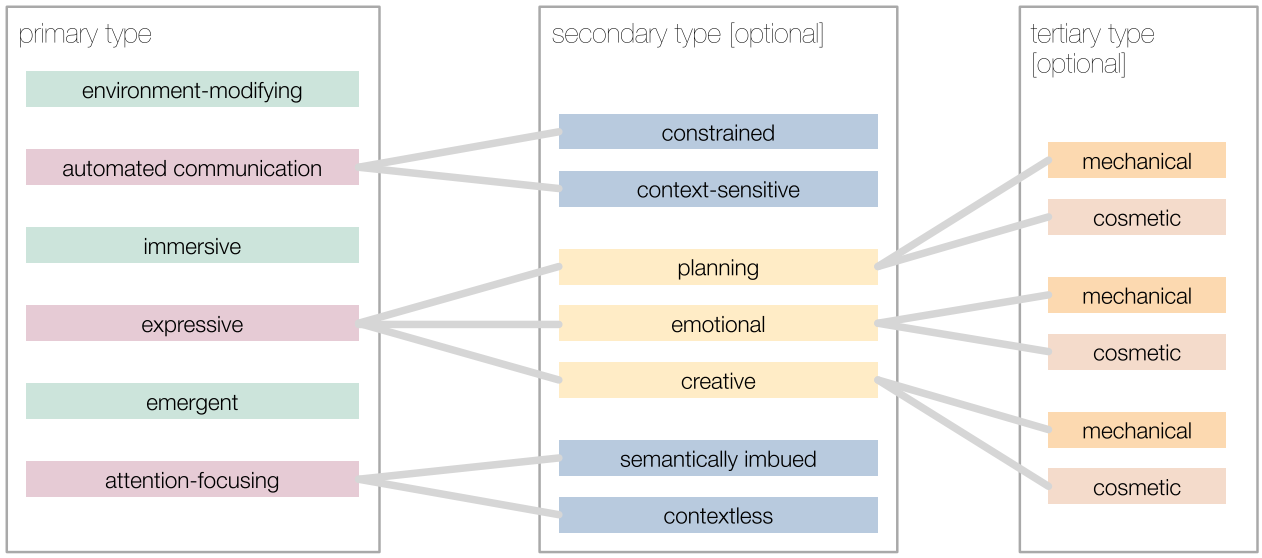
\includegraphics[scale=0.5]{images/framework_cooperative_communication_mechanics.png}
    \caption{\textcite{Toups2014ATheory}[259] divided their framework into up to three levels of classification for game mechanics.}
    \label{fig:framework_cooperative_communication_mechanics}
\end{figure}

\subsubsection{Environment-modifying}
\label{section:Environment-modifying}

Environment-modifying game mechanics allow players to permanently or semi-permanently change some component of the game world to convey information to other players \autocite{Toups2014ATheory}[259].
This reaches from creating signs for an indicated path, other players or the player themselves can follow, to the possibility to create lore created by players, which can merge with the game world. The investigation of \textcite{Toups2014ATheory}[260] showed, that although they can be used to grief or troll players, there are interesting environment-modifying mechanics.
For future help, they could be used to provide information to future players to guide them trough a labyrinth.

Signposts are one of \textcite{Toups2014ATheory}[260] exemplar mechanics, which generally involves players to take a break from other gameplay to interact with a messaging sub-system. Other players on the other hand have to pause their current goal too, to read the sign. This mechanics also do not have to be synchronous.
Players do not need another player to be online. The sign could be placed one week before a player finds it and the message can still be passed to the player. \textcite{Cheung2012CommunicationGaming}[260] mentions the signpost mechanics in \textit{Dark Souls} and \textit{Dark Souls II}, where players can leave messages on the ground, as well as \textit{Minecraft}, which allows players to create signs with short text messages. These signposts are permanently placed, as long as a player does not remove it. As Minecraft allowed players to create buildings, bridges and so on with block-sized voxels, players are also able to create allow-like shapes, which are also count as an environment-modifying mechanic.


\subsubsection{Automated communication}
\label{section:Automated communication}

Automated communication is divided into constrained and context sensitive mechanics.
Constrained automated communication mechanics take the form of pre-defined announcements or responses that the player invokes to explicitly indiate somthing to teammates \autocite{Toups2014ATheory}[260].

"Message Macros" allow the player to efficiently select from a limited set of pre-generated messages and share them with teammates. Instead of typing whole messages into the chat, a player can send messages by a combination of buttons.
The Games Tribes\footnote{\url{https://web.archive.org/web/20151028195605/http://www.hirezstudios.com/tribesascend/home} - accessed on 13th June 2020}, a fast team-based first person shooter, as well as Smite\footnote{\url{https://www.smitegame.com} - accessed on 13th June 2020}, a 5 VS 5 player strategy game, implemented a Voice Guided System (VGS). To warn teammates about a missing enemy in the left game-area, a player in Smite can type \textit{VF1}\footnote{\url{https://smite.gamepedia.com/VGS_Cheat_Sheet} - accessed on 13th June 2020}. This sends the message "Enemy missing left!" to the text-chat and plays a voice-recorded audio feedback to all team members.
Another (corner) case is the possibility to sing in \textit{Journey\footnote{\url{https://thatgamecompany.com/journey/} - accessed on 13th June 2020}}. It is the only communication mechanic and allows the player to interact with the environment and allows other players to locate the game character. Additionally it is counted to being an emergent communication mechanic \autocite{Toups2014ATheory}[261].


Context-Sensitive automated communication mechanics rely on state to parameterize a communication to teammates \autocite{Toups2014ATheory}[261]. It simplifies the exchanging of information between players by allowing players to share information, which seems to be understood by the game itself.
Contextual macros are sending pre-defined information to other players, regarding the currently selected item. In \textit{Diablo III\footnote{\url{https://eu.diablo3.com/de/} - accessed on 13th June 2020}}, a player is able to send the description of a piece of treasure to allies, which normally is only visible to the player who is carrying the item \autocite{Toups2014ATheory}[261].

Context-sensitive automated communication however is more limited, because they this mechanics need to be well planned by the designer. They are only usable in A specific context and may be not usable for the player, when the function in an unfamiliar way \autocite{Toups2014ATheory}[261]. 


\subsubsection{Immersive}
\label{section:Immersive}

Immersive communication mechanics invite teammates to join a shared experience, rather than directing other players towards a specific game-winning behaviour \autocite{Toups2014ATheory}[261].
Immersive mechanics are connected to the game-character and improves the experience within the game. The perfect example for immersive mechanics are character emotes. The player character can act on their own by showing a laughing, dancing or waving animation. But also interactions such as high-fives or playing rock-paper-scissors in \textit{Portal 2\footnote{\url{https://store.steampowered.com/app/620/Portal_2/} - accessed on 30th January 2020}} between multiple players are possible.

\subsubsection{Expressive}
\label{section:Expressive}
 Expressive communication mechanics support players in sharing information about themselves, as well as planning and sharing emotions or to be creative \autocite{Toups2014ATheory}[261]. They are more deeply classified by whether they enact state change on the game or if they are only cosmetic \autocite{Toups2014ATheory}[261].


Expressive planning communication mechanics are used to direct teammates to future gameplay. This includes situational holding mechanics, like holding a weapon. In open-world survival games like \textit{Rust\footnote{\url{https://rust.facepunch.com/} - accessed on 13th June 2020}} or DayZ\footnote{\url{https://dayz.com/} - accessed on 13th June 2020} showing a weapon can indicate that the player is ready for combat and running around without weapons can indicate peace. As \textcite{Toups2014ATheory}[262] notices, this behaviour works because it gives a player a clear disadvantage when violence erupts. Therefore the current equipment is connected to the trust players have towards their teammates and opponents.


Expressive emotional mechanics gives the player the possibility to express themselves to their team. \textcite{Toups2014ATheory}[262] said that expressing their emotions via communication mechanics, positive emotions could cascade through the team when they are shared with them. Gesture mechanics are an example, as an character animation like a thumb-up or trying to hug another player can indicate happy emotions. This animations are often either triggered by writing a text-command into the chat or by any kind of button combination. In \textit{Portal 2} it is possible for a player to give their teammates a high-five, to cheer a successful action together. As these animations have to be pre-defined, players are limited to a selection of gestures provided, but do not have to articulate how they feel in words \autocite{Toups2014ATheory}[262].

\textcite{Toups2014ATheory} do not give any example for creative expressive communication mechanics. Being able to draw images onto walls could be a combination between environment-modifying and creative expressive mechanic, as players are able to express themselves through a cosmetic way to communicate with other players.


\subsubsection{Emergent}
\label{section:Emergent}

Emergent cooperative communication mechanics seem to be different from other mechanics, because they are not necessary implemented to give players the opportunity to communicate with it. They communication with this mechanics exists between certain communities and have to be learned \autocite{Toups2014ATheory}[262]. One example many games have implemented is the possibility to jump, which in the first place is implemented because of movement reasons. However, jumping without any reason can have a semantic meaning, which can mean nearly everything, starting from "Pay attention to me" to "I am impatient" \autocite{Toups2014ATheory}[262]. 
The player community of Smite developed the act of jumping around together with enemy players before the match started as a good sign of will and to wish every player luck and fun. This behaviour is not intended by the game designers and new players do not know about it, unless they read about it or it is explained by another player.

\subsubsection{Attention-focusing}
\label{section:Attention-focusing}

Attention-focusing game mechanics provides players the possibility to gain attention, point onto objects other players should focus on or to give commands, teammates should follow. Giving teammates a description where they need to look at can be more difficult than pointing at it. There are two different types of attention-focusing mechanics, which are either bound to a specific context ore are context-less \autocite{Toups2014ATheory}[262].


A well known communication mechanic is the ping mechanic. Players can click onto the map to create a icon in the virtual game space. Some games combine these with an sound effect to gain the attention of the player, who may look at a different part of the environment.
The most prominent games which provide pings a strategy games, where the position can of characters can have an important value. In strategy games from the \textit{Starcraft\footnote{\url{https://starcraft2.com/de-de/} - accessed on 13th June 2020}} or \textit{Warcraft\footnote{\url{https://playwarcraft3.com/de-de/} - accessed on 13th June 2020}} series, players can ping on the environment or mini-map, which is displayed on their and their allies screen \autocite{Toups2014ATheory}[]263]. The ping itself however has no greater meaning and only highlights a certain position. The purpose of the ping itself needs to be communicated or is understood by all parties through previous experiences.


Attention focusing communication game mechanics can have a semantically imbued meaning, which provides information or carry along commands. \autocite{Toups2014ATheory}[263].
In \textit{League of Legends\footnote{\url{https://leagueoflegends.com/} - accessed on 13th June 2020}} pings can be context-less, but can also be "Augmented environment Pings". The game contains structures such as allied and enemy towers. Clicking on different parts of the game words creates different pings. By creating a ping at the enemy tower, instead of a normal ping with a blue dot, a ping with an red exclamation point appears above the target \autocite{Toups2014ATheory}[263]. Next to the function of pointing at different positions, these augmented pings can tell teammates to defend or attack a certain character or structure.

In \textit{Portal 2} it is possible to choose between different types of pings. Next to a simple "look at"-ping, there are also pings with different icons to indicate that at this position a partner should create a portal. For time-based interactions there is also a countdown-ping, which can improve time-based actions a lot, even with out verbally communicating with each other.


\section{Implementation}
\label{section:Implementation}
The aim of this thesis is to find out, how players interact with each other, while they cannot rely on direct verbal communication channels.
For this reason, a prototype of a cooperative multiplayer game is created.
For the implementation of the game, the game engine Unity\footnote{\url{https://unity.com/}}
is used. 
For the network part, the network engine Photon\footnote{\url{https://www.photonengine.com/}} is used. Photon provides an SDK called Photon PUN, which is an integration for the Unity engine.
The following sub chapters describes the game idea, how the gameplay part is implemented, as well as which and how the communication tools are implemented.



\subsection{Game idea}
\label{section:Game idea}
As the purpose of this game is the testing of communication tools, which are implemented within the game, a simple game is created.
For good cooperation, it was decided to create a cooperative multiplayer game with puzzle elements. The puzzle elements have the purpose to create cooperative puzzles, which can only be solved when players work together. There are nine levels in total the players can complete. Each level has three candies which the players need to collect. All nine levels need to be completed as fast as possible.

\subsubsection{Game elements}
\label{section:Game elements}

\begin{figure}
    \centering
    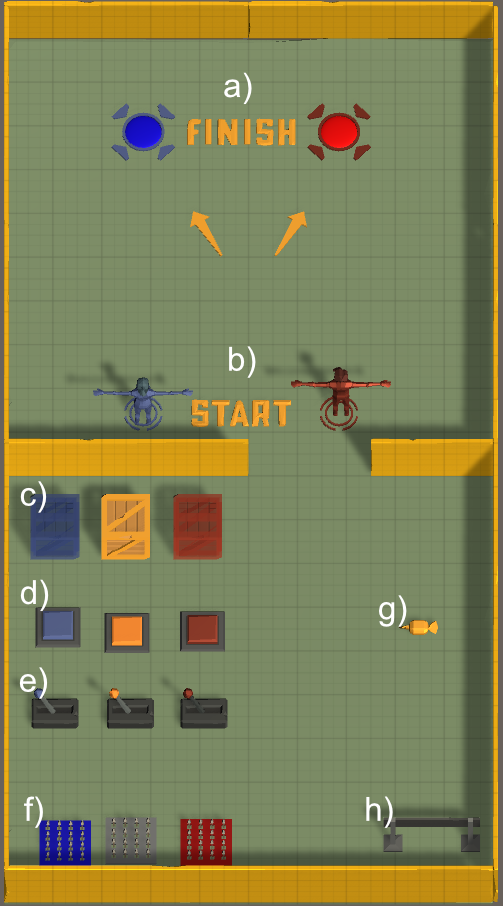
\includegraphics[scale=0.4]{images/lobby_game_elements.png}
    \caption{Overview of all game elements:
    a) goal points for each player b) start points and players c) movable boxes d) pressure plates e) switches f) traps g) candy h) barrier}
    \label{fig:game elements}
\end{figure}


Each level consists of a floor and walls. There are always two spawn-points, one for each player, as well as a goal-point for each player. The next level will load, as soon as both players are standing on their goal-point.


\begin{enumerate}
    \item Candy
    
    In each level there are three candies players are able to collect. Each candy adds one score point to the shared team score.
    \item Movable box:   
    
    The movable box blocks the way of the player. This box can be pulled towards the player or pushed in the forward direction of the player. It is not possible to move it sidewards, so the movements are limited to two directions, according to the player's position.
    \item Barrier
    
    The barrier blocks the player's path like a box. The player themself is however not able to interact with it directly. A barrier can be disabled by other elements such as switches or pressure plates
    \item Switch
    
    A switch has the purpose of enabling or disabling objects. A switch can disable a barrier, so players can pass it.
    It is also possible to enable and disable traps with it.
    
    Some switches are connected together. Both switches will only stay active, when they are activated at the same time.
    \item Pressure Plate
    
    Pressure plates are similar to switches. However, the difference to a switch is that it gets activated while a player is standing on top of it. It is also possible to move a box on top of it, so it will stay active while the both players can move around freely.
    
    There are also pressure plates that are connected with each other. Only while all connected pressure plates are active at the same time, a barrier, for example, is deactivated.
    \item Trap
    
    An active trap pulses between states of extended and retracted spikes. When the trap has retracted spikes, the player is able to move on top of it freely. When the player is on top of the spikes while they are extended, the player is sent back to the start.
\end{enumerate}

The graphics for all listed elements can be seen in Figure \ref{fig:game elements}.

Movable boxes, switches, pressure plates and traps can also have the colour of one player. 
Blue pressure plates can only be activated while the blue player or a blue box is on top of it.
Blue switches can only be activated by the blue player and only the blue player is able to move a blue box.
Even if traps are coloured, both players will respawn when they collide with it.
The same is valid for the red player and red objects

To force the player to collaborate with their partner, a blue object can only be seen by the red player, and a red object can only the seen by the blue player. As both players are not able to see every object they can interact with, they need to tell their partner, where an object is, where a box needs to be moved to and which areas they need to leave untouched.

\subsubsection{Cooperative game mechanics}
\label{Cooperative game mechanics}

To give the players the possibility to interact with each other, there are the following mechanics a player can use.

\begin{figure}[h!]
    \centering
    \begin{subfigure}[b]{0.4\linewidth}
        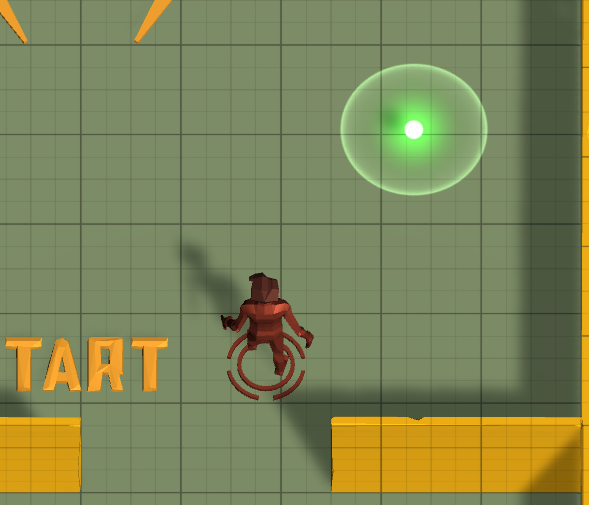
\includegraphics[width=\linewidth]{images/location_ping.png}
        \caption{Location ping}
        \label{fig:location ping}
      \end{subfigure}
    \begin{subfigure}[b]{0.4\linewidth}
        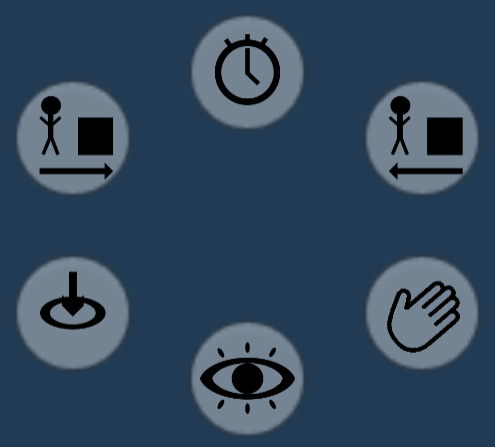
\includegraphics[width=\linewidth]{images/ping_types.png}
        \caption{All six ping types}
        \label{fig:ping types}
    \end{subfigure}
    \caption{
    Different ping indicators.}
\end{figure}

In the game, three types of pings are available. As mentioned in
Section \ref{section:Attention-focusing}, pings are counted towards attention-focusing game mechanics. With a simple left click of the mouse, a location-ping is created at the clicked position. On figure \ref{fig:location ping} a location ping can be seen.
In addition to a simple location-ping, a player can also use six semantically imbued pings. Figure \ref{fig:ping types} shows all six typed a player is able to choose. For time critical actions such as a time based switch, a countdown ping can be placed. The other five options should give the player the possibility to give commands to other players. 


\begin{figure}
    \centering
    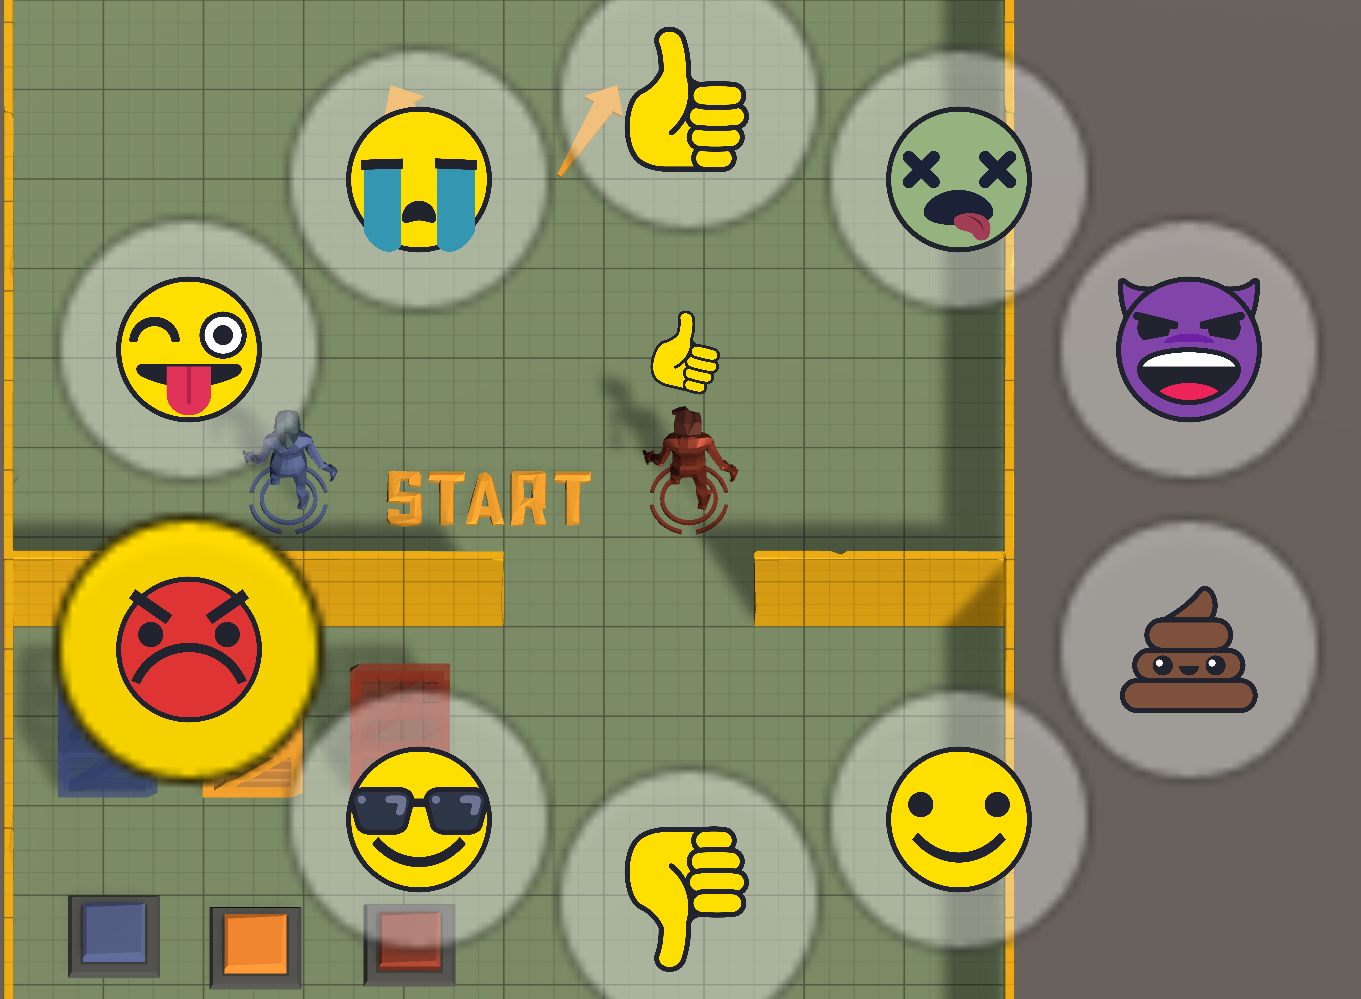
\includegraphics[width=0.5\textwidth]{images/emoji_selection.png}
    \caption{Selection interface of all emojis. A thumbs-up emoji is played above the red player.}
    \label{fig:emoji selection}
\end{figure}

For immersive communication, players get the option to use emojis.
Figure \ref{fig:emoji selection} shows all selectable emojis. The selection window opens while the right mouse button is pressed. The currently selected emoji is chosen when the right mouse button is released by the player.
In addition to all eight selectable emojis, an exclamation mark emoji can be shown above the players head. The intention behind the emojis is to give the player a way to express their feelings. Players should have the possibility to describe their current emotional state without choosing wording. This communication mechanic is a expressive emotional game mechanic as described in \ref{section:Expressive}.


\begin{figure}
    \centering
    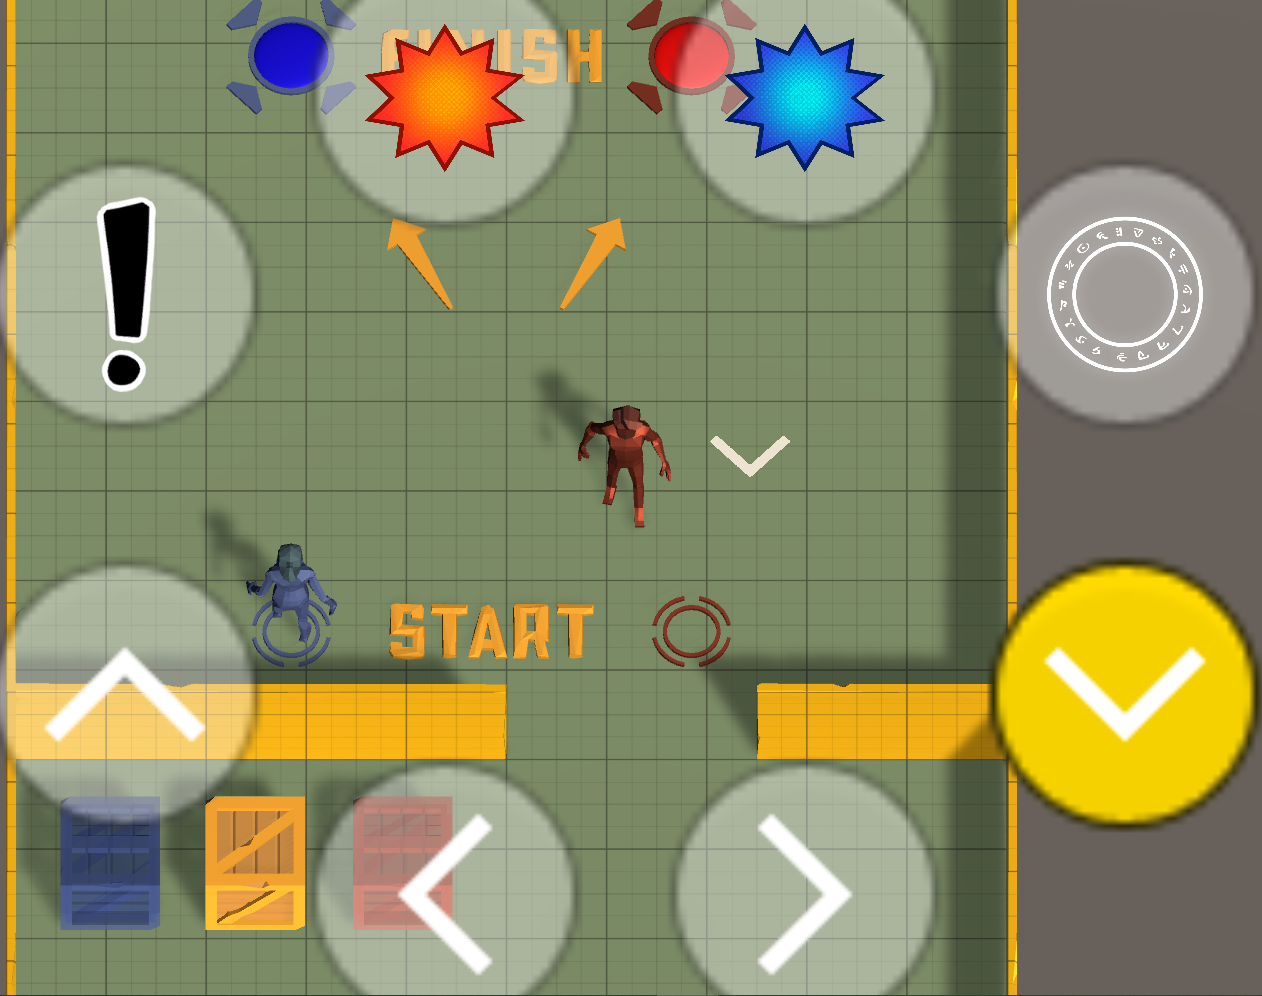
\includegraphics[width=0.5\textwidth]{images/decal_selection.png}
    \caption{Selection interface of all decals.}
    \label{fig:decal selection}
\end{figure}

To create longer lasting messages, players can create decals with eight different images, seen in \ref{fig:decal selection}. This decal-system is an environment-modifying communication mechanic, described in \ref{section:Environment-modifying}. These images are placed onto the ground below the player. Every decal overlaps the last one, but is not deleted. They last as long as the current level is played. With arrow marks on the floor as an example, players could mark a safe path which can be run along.


The fourth communication game mechanic is the recording of the current player position. While pressing the Ctrl-key or the middle mouse button, the current location of the player is saved. On release, a light transparent sphere with the player-colour is following the recorded path. This tool is not necessarily a way to communicate with each other. It was implemented to test, if players would use the ghost for emergent cooperative communication as described in section \ref{section:Emergent}. Theoretically, it could also be used to "draw" signs by walking onto the environment. The main purpose however, is to give the user the possibility to record a safe path they were able to run along.



\subsection{Gameplay implementations}
\label{section:Gameplay implementations}


\subsubsection{Player Character}

Both, the red player and the blue player, have the same scripts and components applied. They only differ by attributes like the player id, the layer to look for interactable objects, as well as the player colour.
The player input is handled via the \textit{Unity Input System\footnote{\url{https://docs.unity3d.com/Packages/com.unity.inputsystem@1.0/manual/index.html} - accessed on 14th June 2020}}. For simplicity, both player characters listen to the player input, but only the character which is controlled by the local player executes the method completly.
Each player character has a \textit{Player}-Script attached with a public method named \textit{CanUsePlayerObject()}, which returns whether the player character is controlled by the local player.

When a player joins the game, the Lobby scene gets loaded by the \textit{NetworkGameManager}. The NetworkGameManager Updates the current player map, which maps all player ids (representing the player colour) to the actor number provided by Photon. The first player is always mapped onto the red player, the second player is controlling the blue player.
The local player actor number, retrieved via \texttt{PhotonNetwork.LocalPlayer.ActorNumber}, can then be checked against the actor number behind a player id.

Per default, only the host, which here is the red player as the first player, is able to control objects. To move objects or the player around, the ownership of the object has to be transferred to the local player, who wants to modify it.
When a level is loaded, the ownership of the player characters are set to the actor number, which is mapped to the corresponding player id.

The character is then moved by the \textit{PlayerMove} script.
The input direction is saved to a corresponding variable, which is updated with an event-call, triggered by an input change. When the player is not trying to move a box, the built-in character-controller is instructed to move the player towards the wanted direction, as long there is no collision detected.
The player is also rotating towards the movement input direction.

By pressing space, the \textit{PlayerInteract}-Script checks for interactable objects in front of the player by using a raycast. If the interactable object is also moveable, which means it is a moveable box, a reference is saved.
While the \textit{PlayerMove}-Script has a reference of a \textit{MoveableObject}, it additionally moves the corresponding object. First, it is checked if the object can be moved in the given direction. When the object returns a positive call, the moveable object and the character is moved.

When the player presses the interaction-key, while a toggle is in front of the player, the \textit{Interact()}-method of the toggle is called.

The \textit{PhotonView}-Component attached to the player character synchronises the player position, rotation and the current animation state among all players.


\subsubsection{Camera}

The camera itself is handled by Unity's \textit{Cinemachine\footnote{\url{https://docs.unity3d.com/Manual/com.unity.cinemachine.html} - accessed on 14th June 2020}}-Framework.
Each scene has a virtual camera, controlled by a \textit{CinemachineVirtualCamera}-script. The local controllable player is set as the follow-target of the \textit{CinemachineVirtualCamera}-script.
Thus the virtual camera transposes the camera to a fixed offset.

\subsubsection{Overlapping Collider}

Overlapping colliders are used by pressure plates and moveable boxes.
When the OnTriggerEnter-Callback is called by Unity's physic engine, it is checked if triggers should be ignored, if the given collider should be ignored and if the overlapping object has an accepted trigger.
When the object is valid, it is added to the currently overlapping collider list. The \textit{IsOverlapping}-Method will return true, if there is a overlapping collider.
One exception exists: If the parameter is also given the player collider, and the player collider is the only collider added to the overlapping collider list, the method is returns false. This was implemented because a character was not able to pull a box object when the character was in range, while moving the object.

\subsubsection{Moveable Box}

Each moveable box has an \textit{OverlappingCollider} attached to each side , as well as a MoveableObject-Script. The \textit{IsMoveable}-Method is called by the \textit{PlayerMove}-Script, when it is set as the referenced \textit{MoveableObject}, as described before. It will return true if the overlapping collider at the required direction is returning no future collision with other objects.
When a Box is already moved by another player, the box will not be interactable until the other player stops the interaction.

\subsubsection{Pressure Plate}

Pressure plates are using an overlapping collider, which checks if there is an object above the pressure plate.
When the enabled state changes, a remote procedure call(RPC) is used to sync the pressure plate among all players.
To be able to use RPCs, a GameObject needs to have a PhotonView-Component.

As each PhotonView-Component has an id, the RPC can be sent and the correct method on the object with the same id on the other machine is called.
When the id of a \textit{PhotonView}-Component has a duplicate without the required method, an error is thrown.
This can occur when the scene has changed and the new scene has network-objects with the same id, but different scripts attached. To bypass this circumstance, Photon has the option to set the minimum id for a scene. Id's below the minimum are updated to the next free id, that is available in the current scene.

When the state is changed by an incoming RPC-Call, \textit{UnityEvent}s for enabling and disabling pressure plates are invoked. As a result, the \textit{UnityEvent} can be used in the inspector, to enable or disable objects or call public methods.

\subsubsection{Toggle}

Toggles work similar to pressure-plates but have a simple \textit{Interactable}-method, called by the PlayerInteract-Script when the player stands in front of a toggle. The state is always flipped and sent via an RPC, to synchronise all toggles.


\subsubsection{Sync-Toggle}

Sync-Toggles can only be indirectly manipulated by the player.
Sync-Toggles have elements, which can be enabled and disabled by pressure-plates or toggles. Sync-Toggles are activated when all elements are enabled. The goal-platform is a special sync-toggle which loads the next level when both players are standing on their corresponding goal-pressure plate.
When an element is enabled or disabled, an RPC is called.
The UnityEvents are only invoked when the state has changed, to prevent an RPC-loop between sync-toggles and other toggles, which are connected to each other.

Sync-Toggles can be time-critical. When not all elements are activated at the same time (with a maximum time-offset of 0.2 seconds), the elements are disabled again, which results in toggles which turn themselves off again.

\subsubsection{Traps}

Traps consist of a parent \textit{TrapCollection}-Object, which contains one or multiple Trap-objects and multiple \textit{Trap}-Objects attached to the \textit{TrapCollection}-Object.
When the trap-collection is enabled, a coroutine enables and disables all child-traps. When a player collides with the trigger of a trap, the trap will add the player to the respawn-list of the \textit{PlayerSpawnController}. This only occurs to the local player to prevent respawning because of asynchronous traps between games and network delay.


\subsection{Implemented cooperative game mechanics}
\label{section:Implemented cooperative game mechanics}

\subsubsection{UI Selection Canvas}

To give the player multiple options for pings, emojis and decals, a selection user interface is necessary. The UI is not directly bound to the game mechanics. Instead the ping, emoji and decal mechanics all use their own instance of an UI selection.
Each game mechanic can enable its corresponding UI selection canvas.

\begin{figure}
    \centering
    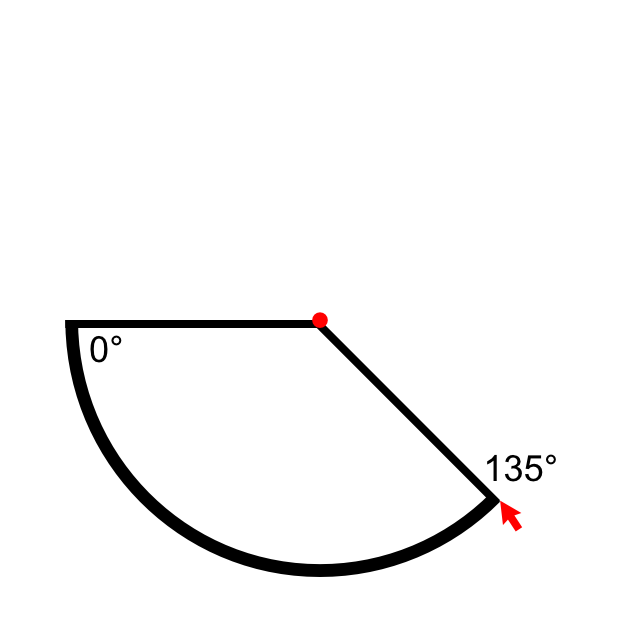
\includegraphics[width=0.5\textwidth]{images/angle_calculation.png}
    \caption{The screen angle is calculated around the centre of the screen, marked by the red dot. The red arrow symbolises the current mouse position. With these two coordinates, the screen angle is calculated using an arc-tangent function.}
    \label{fig:angle calculation}
\end{figure}

Every Canvas has a GameObject with a \textit{SelectionUI}-Component. The corresponding game mechanic implementation updates the current angle, which is used to enable the background of the selected object. The angle can be seen in Figure \ref{fig:angle calculation}. A two dimensional vector, starting from the centre of the screen to the current mouse position, is used to calculate the current screen angle in degrees.

\begin{lstlisting}[
	label=listing:Main, %for reference to this listing
	float=h,
	caption=GetScreenAngle() calculation,
	firstnumber=10
]
    private float GetScreenAngle()
    {
        var screenMiddle = new Vector2(Screen.width * 0.5f, Screen.height * 0.5f);
        var direction = this.currentMousePos - screenMiddle;
        var angle = Mathf.Atan2(direction.y, direction.x);
        angle *= Mathf.Rad2Deg;
        angle += 180;

        return angle;
    }
\end{lstlisting}

A background-GameObject is assigned to a range between two angles. The GameObject is enabled when the angle is set to a value within the range, corresponding to the GameObject.



\subsubsection{Ping implementation}

To place a ping, a raycast from the camera towards the clicked object is created, by using a ray from the camera and its looking direction by using the \textit{ScreenPointToRay()}-Method on the camera-component. When the left mouse button is pressed down, the current mouse position is saved. Using this position as a parameter for \textit{ScreenPointToRay()}, a hitpoint is calculated. This hit point is used as the position for the ping placement.

When the left mouse button raises again within 0.2 seconds, the standard ping is placed. After this period, the selection UI is enabled and by using the calculated screen angle, which is also parsed to the selection UI, a special ping is placed. This placement is done by an RPC, which has a 3D vector for the position, as well as the angle value as parameters.

Default and special pings are both particle systems with an \textit{PingElement}-Script.
When the placement RPC for a ping is received, the ping object chosen with the angle if it is a special ping. Otherwise the next standard ping from a circular buffer is taken. To place the ping object, the \textit{PingElement}-Script has a \textit{PingAt(position)}-Method, which places the object and starts to play the particle effects.

\subsubsection{Emoji implementation}

Emojis are created with the right mouse button. Like the ping-tool, the emoji-tool also has a standard-emoji for a short press, which is an exclamation mark.
When the right mouse button is pressed over 0.2 seconds, the emoji selection UI is enabled, and the player can choose from 8 different emojis by using their mouse position.

The GameObjects with a particle system for each emoji are children of the player object.
Each player object has a \textit{PlayerEmote}-Script, which gets called by the emote-tool on receiving an RPC. As the angle and the player id are sent along as parameters, so the emoji starts playing above the right player.

\subsubsection{Decal implementation}

The decal system selection UI is enabled as soon as the \textbf{F}-key is pressed down. The screen angle is used to choose from the available decals. When the RPC is sent, the current player position is sent along for the placement of the decal.

On receiving the RPC, the decal corresponding to the angle parameter is placed on the position plus an offset on the y-coordinate. With this offset, it is possible to overlap decals without removing the old one.

\subsubsection{Ghost implementation}

While the middle mouse button or Ctrl-Key is pressed, the position of the character is saved in an array of positions with an time-step of 0.1 seconds. The limit for the recording is set to 100 recording steps, which is equal to around 10 seconds.
When the record-key is released, the player id and the array of positions is sent using an RPC.

On receiving the call, a ghost is selected using the player id and is given all position steps. The ghost will then circle through the positions with an coroutine. When the first position is selected, it is placed onto it, otherwise the next target position is saved. 

Using the next target position, the ghost will move towards its direction with the same movement speed of the player. To create the illusion of a hovering ghost, the coloured sphere's y-coordinate is also changed using a sine wave. This will move the sphere mesh up and down within a range from -0.2 to 0.2 units. One sine wave has a duration of 5 seconds.



\newpage
\subsection{Implemented level layouts}
\label{section:level layouts}

\begin{figure}[h!]
    \centering
    \begin{subfigure}[b]{0.45\linewidth}
        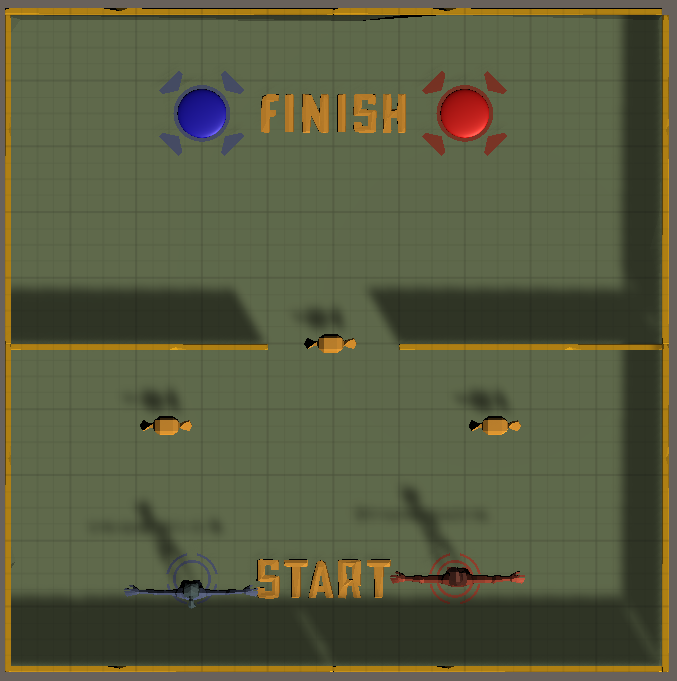
\includegraphics[width=\linewidth]{images/level_1.png}
        \caption{Level 1}
        \label{fig:level 1}
      \end{subfigure}
    \begin{subfigure}[b]{0.45\linewidth}
        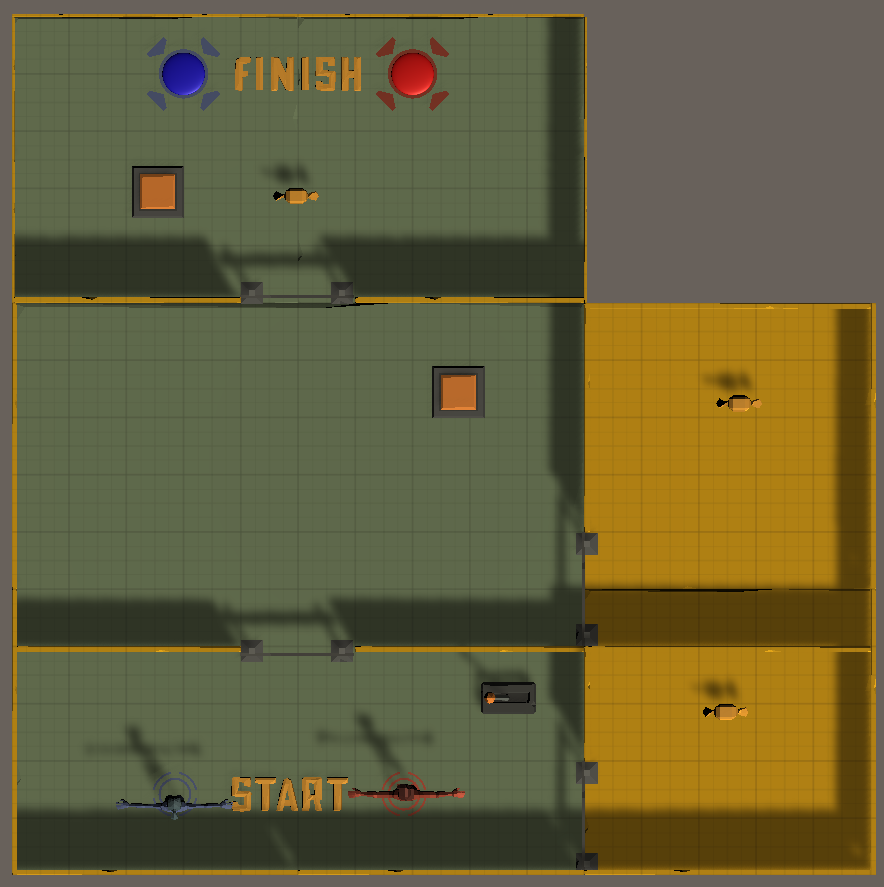
\includegraphics[width=\linewidth]{images/level_3.png}
        \caption{Level 3}
        \label{fig:level 3}
      \end{subfigure}
    \begin{subfigure}[b]{0.45\linewidth}
        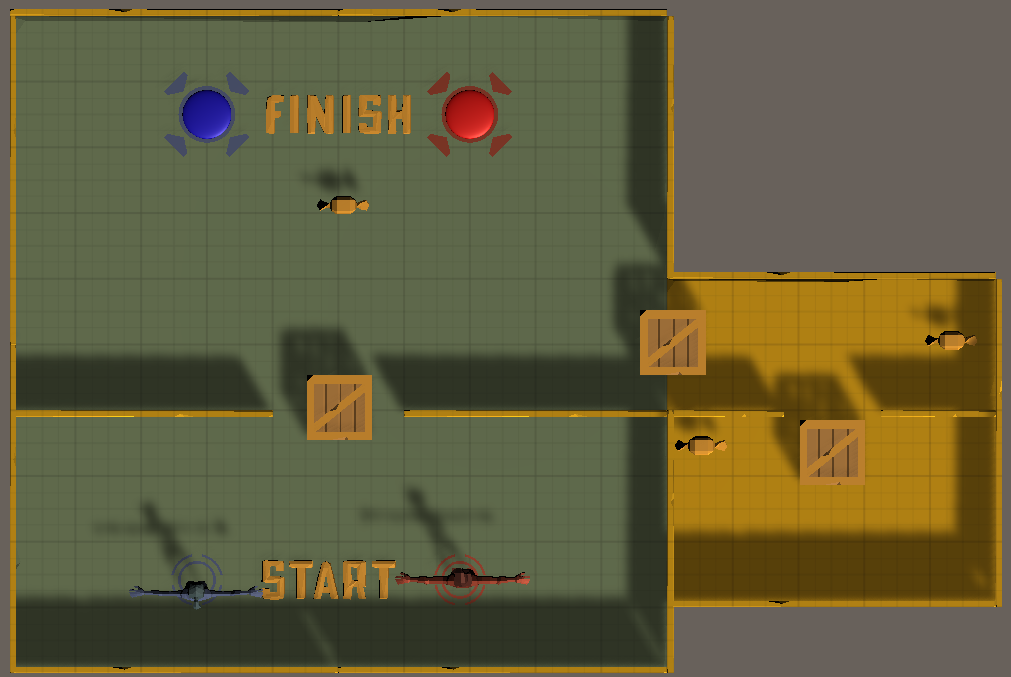
\includegraphics[width=\linewidth]{images/level_2.png}
        \caption{Level 2}
        \label{fig:level 2}
      \end{subfigure}
    \begin{subfigure}[b]{0.45\linewidth}
        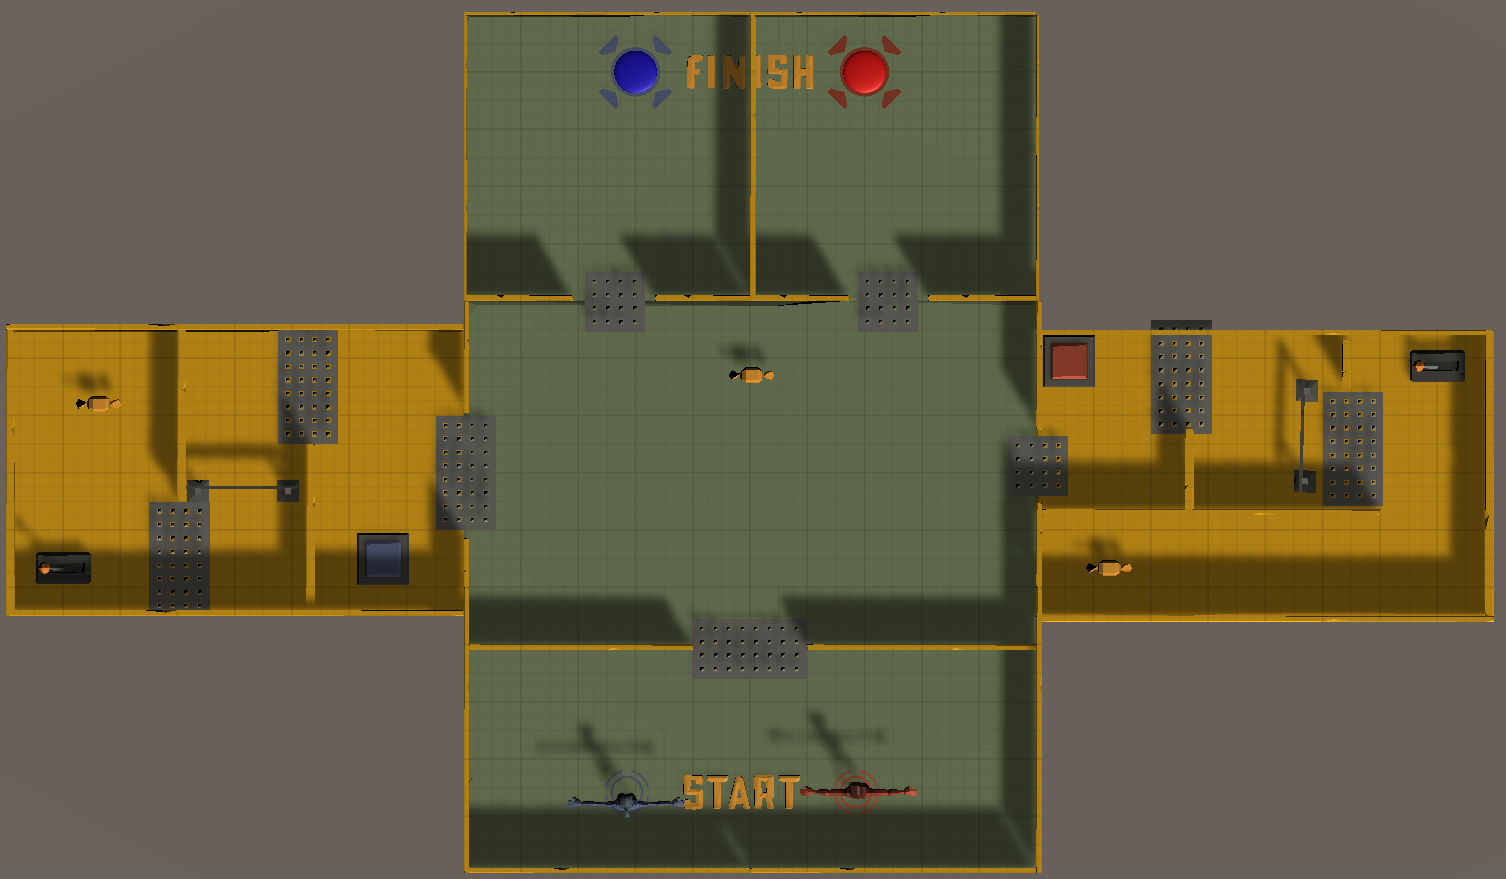
\includegraphics[width=\linewidth]{images/level_4.png}
        \caption{Level 4}
        \label{fig:level 4}
      \end{subfigure}
    \begin{subfigure}[b]{0.45\linewidth}
        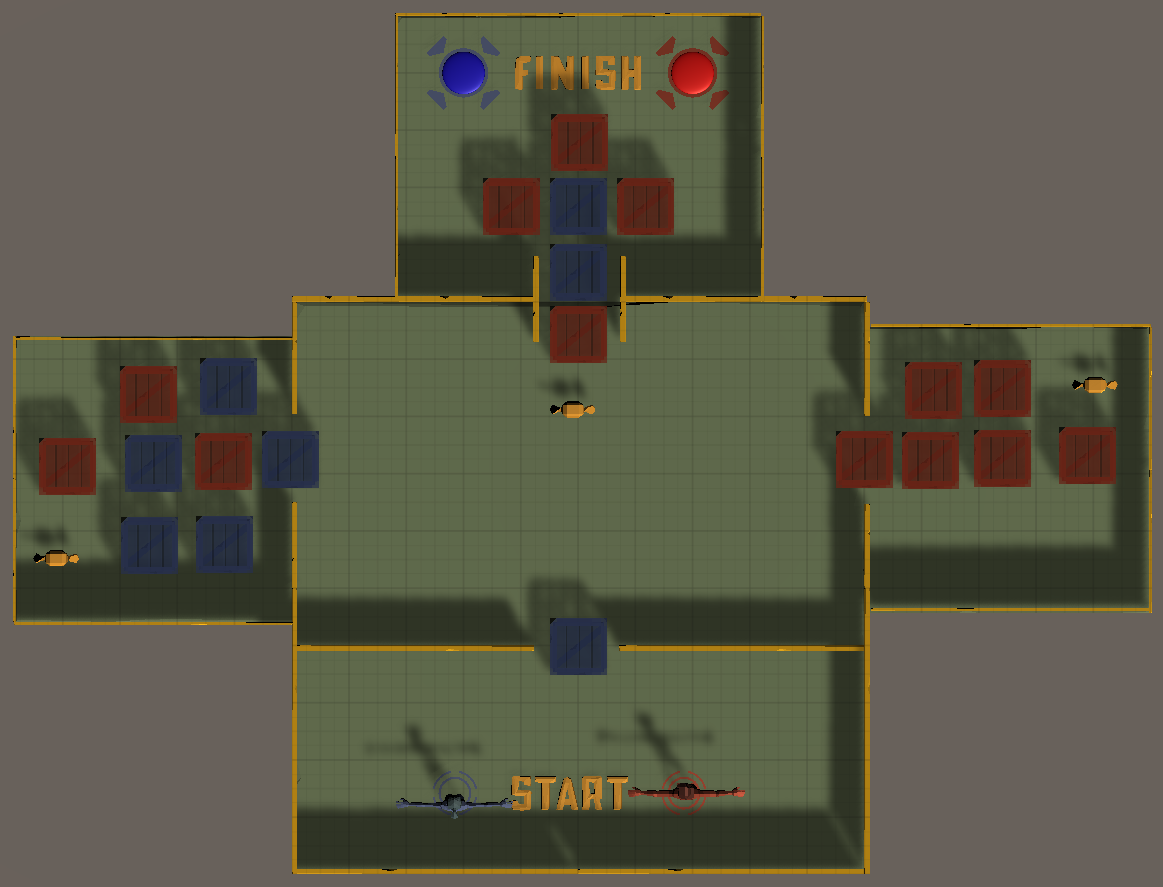
\includegraphics[width=\linewidth]{images/level_5.png}
        \caption{Level 5}
        \label{fig:level 5}
      \end{subfigure}
    \caption{Level 1-5}
\end{figure}


\newpage
\begin{figure}[h!]
    \centering    
    \begin{subfigure}[b]{0.45\linewidth}
        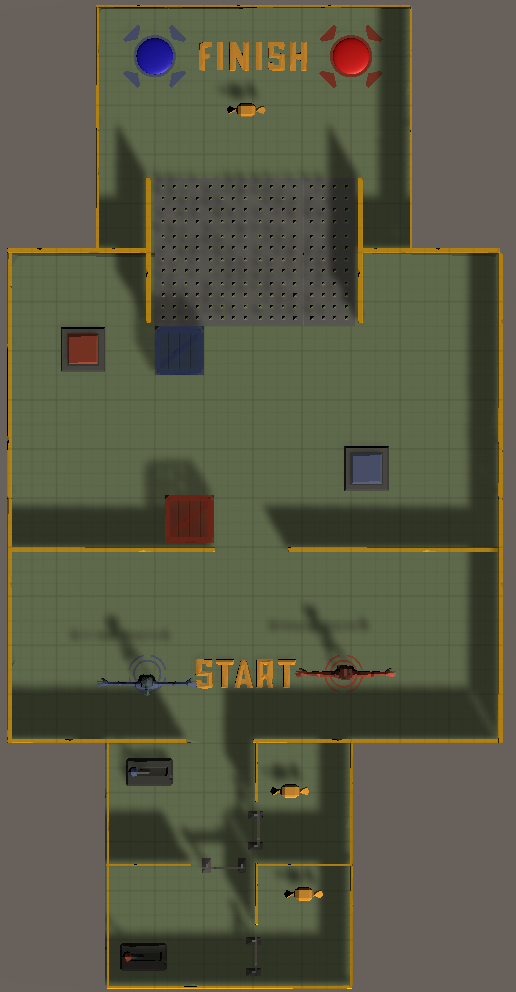
\includegraphics[width=\linewidth]{images/level_6.png}
        \caption{Level 6}
        \label{fig:level 6}
      \end{subfigure}
    \begin{subfigure}[b]{0.45\linewidth}
        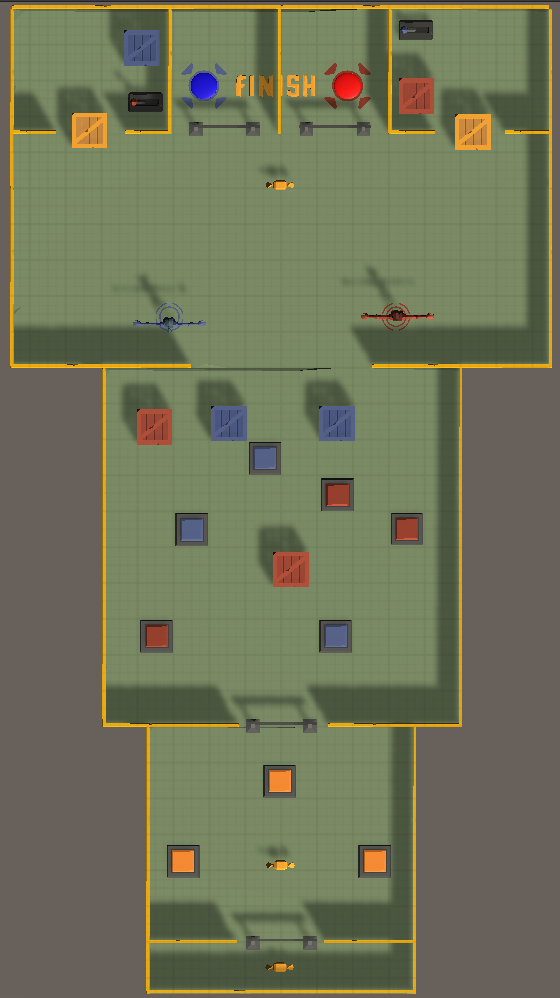
\includegraphics[width=\linewidth]{images/level_8.png}
        \caption{Level 8}
        \label{fig:level 8}
      \end{subfigure}
    \begin{subfigure}[b]{0.45\linewidth}
        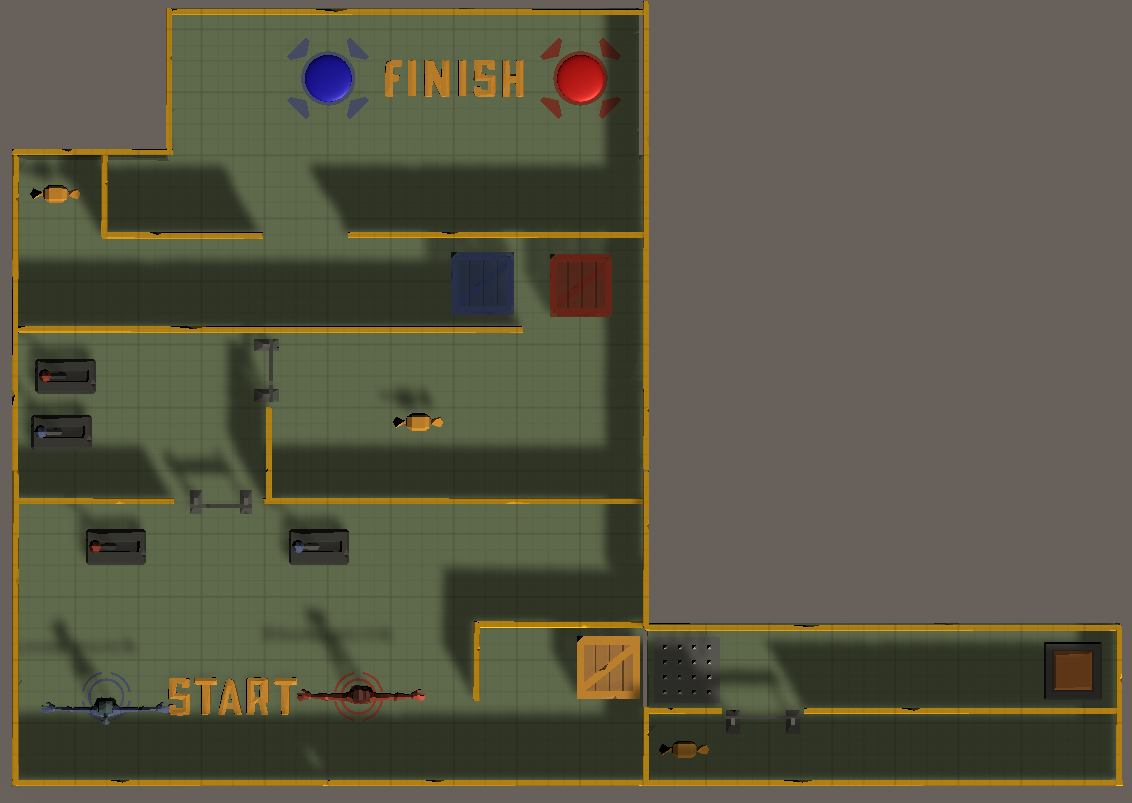
\includegraphics[width=\linewidth]{images/level_7.png}
        \caption{Level 7}
        \label{fig:level 7}
      \end{subfigure}
    \begin{subfigure}[b]{0.45\linewidth}
        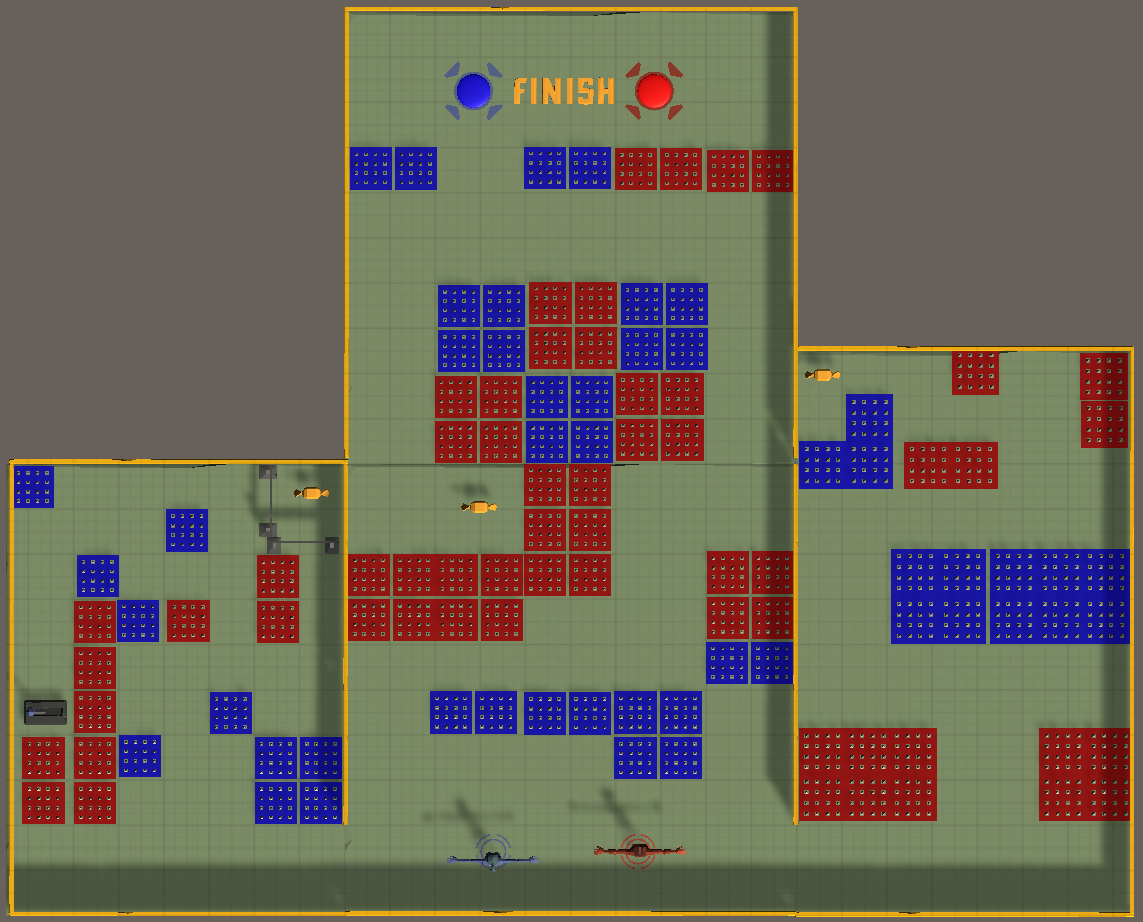
\includegraphics[width=\linewidth]{images/level_9.png}
        \caption{Level 9}
        \label{fig:level 9}
      \end{subfigure}
    \caption{Level 6-9}
\end{figure}

\section{Study}
\label{section:Study}
The whole study was completed online.
Every participant was sent an informed consent form and privacy policy, which was read, signed and returned by everybody.
Discord\footnote{\url{discordapp.com/} - accessed on 21th June 2020} was ised as a communication software. The participants registered as a team of two. 
Every team was added to a private discord group, which allowed screen sharing from multiple attendees.

At the start of each test, the participants received access to the game, which was downloaded on their personal computer.
Every participant shared their screen showing the game. The conference and the screen share was recorded for an analysis afterwards using OBS Studio\footnote{\url{https://obsproject.com/} - accessed on 21th June 2020}.
After both players started the game, the lobby was used to explain how the controls of the game worked, how they could interact with objects and what the goal of the game was. They were also told, that objects with the same colour would be invisible for them, and their partner would have the duty to instruct them without verbal communication.
All built-in communication tools were described and remaining gameplay-questions answered.

Each participant had to mute their microphone to prevent any verbal communications and the discord window was minimised to prevent the unintended disclosure of information by looking at the screen of the partner.
The team started the first level afterwards. All nine levels had to be absolved without a break in between.
After each team reached the goal, they were asked following questions:

\begin{enumerate}
    \item How would you rate your experience with computer games, on a scale of one to five, where five means you have a lot of experience?
    \item How would you rate your experience with cooperative computer games, on a scale of one to five, where five means you have a lot of experience?
    \item How old are you?
    \item What is the relationship to your partner?
    \item How long have you known your partner?
\end{enumerate}

Additionally, there was an open question about what they missed by using these communication tools.
The log-files of each participant were transmitted for later analysis.
Afterwards, the participation was completed.

Each log-file contained the amount of usage for:
\begin{itemize}
    \item standard pings
    \item special pings
    \item standard emotes
    \item special emotes
    \item placed decals
    \item recorded ghosts
\end{itemize}

The recorded footage was used to analyse the reason why interactions were used and how long every team needed to complete a level.


\section{Evaluation}
\label{section:Evaluation}
Afterwards, a evaluation part will describe the results of the study
and how these information-providing arrangements are influencing the player performance and
their teamwork in cooperation games.


\section{Conclusion}
\label{section:Conclusion}
In this study, I analysed how non-verbal communication mechanics could be implemented in a small cooperative puzzle game. Furthermore, the study showed, how these implemented mechanic were used by the participants.

With this study, no causal relation between the duration or the type of relationship could be found. 
A study with a higher amount of participants could show better results regarding this.
Also, a higher variety of experienced players could show more different usages of the implemented mechanics, as well show how often these are needed. 
As every player had a lot of experience, inexperienced players may handle the communication different, therefore a study with more participants having different skill-levels would be a topic for the future.

However, the study proved, that it is possible to communicate in new virtual worlds, without any arrangements concerning the usage of how the tools are used. Nevertheless, it also showed that a missing common ground and not having the possibility to build up a common ground, a lot of misinterpretation occurred during the communication.
\textcite{Vaddi2016Investigating2}[46] stated that the performance of teams using a combination of voice and mechanics were significantly faster, which could be related of having the possibility to negotiate tactics and usage of tools and therefore building up their common ground.

Besides the misinterpretation, three teams also stated that they were missing the possibility to show, that they had no clue what to do, and what the other player meant. For that reason, they would like to have a question mark or thinking-emoji to signal their partner about their concerns.
Another thing three teams mentioned, are the possibility to cancel interactions. One a button was clicked, there was no way to cancel, whereby unwanted communication actions were influencing the study with unwanted and unnecessary interactions. They also stated, that not having a possibility to cancel the mechanic, was annoying to them, especially when they were confusing the key-binding to the wanted tool.

When these methods are implemented in a real game, it also have to be considered, which different options players should have. Some options of emojis and decals were simple not used, as well as the pull & pushed ping could have been combined into a single option. As too many choices can slow down the search for a specific option, as stated by two participants, having more play-tests to find the optimal amount of choices is highly recommended. % the main text

%\input{acknowledgements}

\ifmmtpaper

\printbibliography

\else % only use the following for thesis format

\newpage
\printbibliography

\fi


 % group open
\ifmmtpaper 
\begingroup 
    % is required because paper template messes with sizes
    \fontsize{12}{18}\selectfont        
    \setlength{\parindent}{0pt}
    \setlength{\parskip}{5pt plus 2pt minus 1pt}
    \sectionfont{\fontsize{14}{15}\selectfont}
\fi

\newpage
\onecolumn
\begin{appendices}

%\renewcommand{\thesubsection}{\Alph{subsection}}

\section{git-Repository}

Prototype repository: \url{https://gitlab.mediacube.at/fhs41026/ba2-game}

Thesis repository: \url{https://gitlab.mediacube.at/fhs41026/bachelorarbeit-2/}

\section{List of Abbreviations}

CVE: Collaborative Virtual Environment

FPS: First Person Shooter

MOBA: Multiplayer Online Battle Arena

UI: User Interface

RPC: Remote Procedure Call

VGS: Voice Guided System

VoIP: Voice over Internet Protocol

\section{Archived Websites}
% \show\UrlBreaks
\sloppy

\url{https://web.archive.org/web/20200621223303/https://store.steampowered.com/app/620/Portal_2/}, last access on 28th June 2020

\url{https://web.archive.org/web/20200621223319/https://store.steampowered.com/app/570/Dota_2/}, last access on 28th June 2020

\url{https://web.archive.org/web/20200624193804/https://www.smitegame.com/}, last access on 28th June 2020

\url{https://web.archive.org/web/20190610081655/https://smite.gamepedia.com/VGS_Cheat_Sheet}, last access on 28th June 2020

\url{https://web.archive.org/web/20200616093013/https://thatgamecompany.com/journey/}, last access on 28th June 2020

\url{https://web.archive.org/web/20200522045755/https://eu.diablo3.com/de/}, last access on 28th June 2020


\url{https://web.archive.org/web/20200624215328/https://rust.facepunch.com/}, last access on 28th June 2020

\url{https://web.archive.org/web/20200622015819/https://dayz.com/}, last access on 28th June 2020

\url{https://web.archive.org/web/20200504140328/https://starcraft2.com/de-de/}, last access on 28th June 2020

\url{https://web.archive.org/web/20200411081556/https://playwarcraft3.com/de-de/}, last access on 28th June 2020

\url{https://web.archive.org/web/20200626090400/https://leagueoflegends.com/}, last access on 28th June 2020

\url{https://web.archive.org/web/20200628142410/https://unity.com/}, last access on 28th June 2020

\url{https://web.archive.org/web/20200617230437/https://www.photonengine.com/}, last access on 28th June 2020

\url{https://web.archive.org/web/20200430020838/https://docs.unity3d.com/Packages/com.unity.inputsystem@1.0/manual/index.html}, last access on 28th June 2020

\url{https://web.archive.org/web/20200628190656/https://docs.unity3d.com/Manual/com.unity.cinemachine.html}, last access on 28th June 2020

\url{https://web.archive.org/web/20200626080639/https://discordapp.com/}, last access on 28th June 2020

\url{https://web.archive.org/web/20200625011743/https://obsproject.com/}, last access on 28th June 2020

\end{appendices}


% group closing
\ifmmtpaper
\endgroup
\fi


\end{document}
